\documentclass[tikz,border=8pt]{standalone}
\usepackage{amsmath,amssymb}
\usetikzlibrary{arrows.meta,automata,positioning,quotes}
\begin{document}
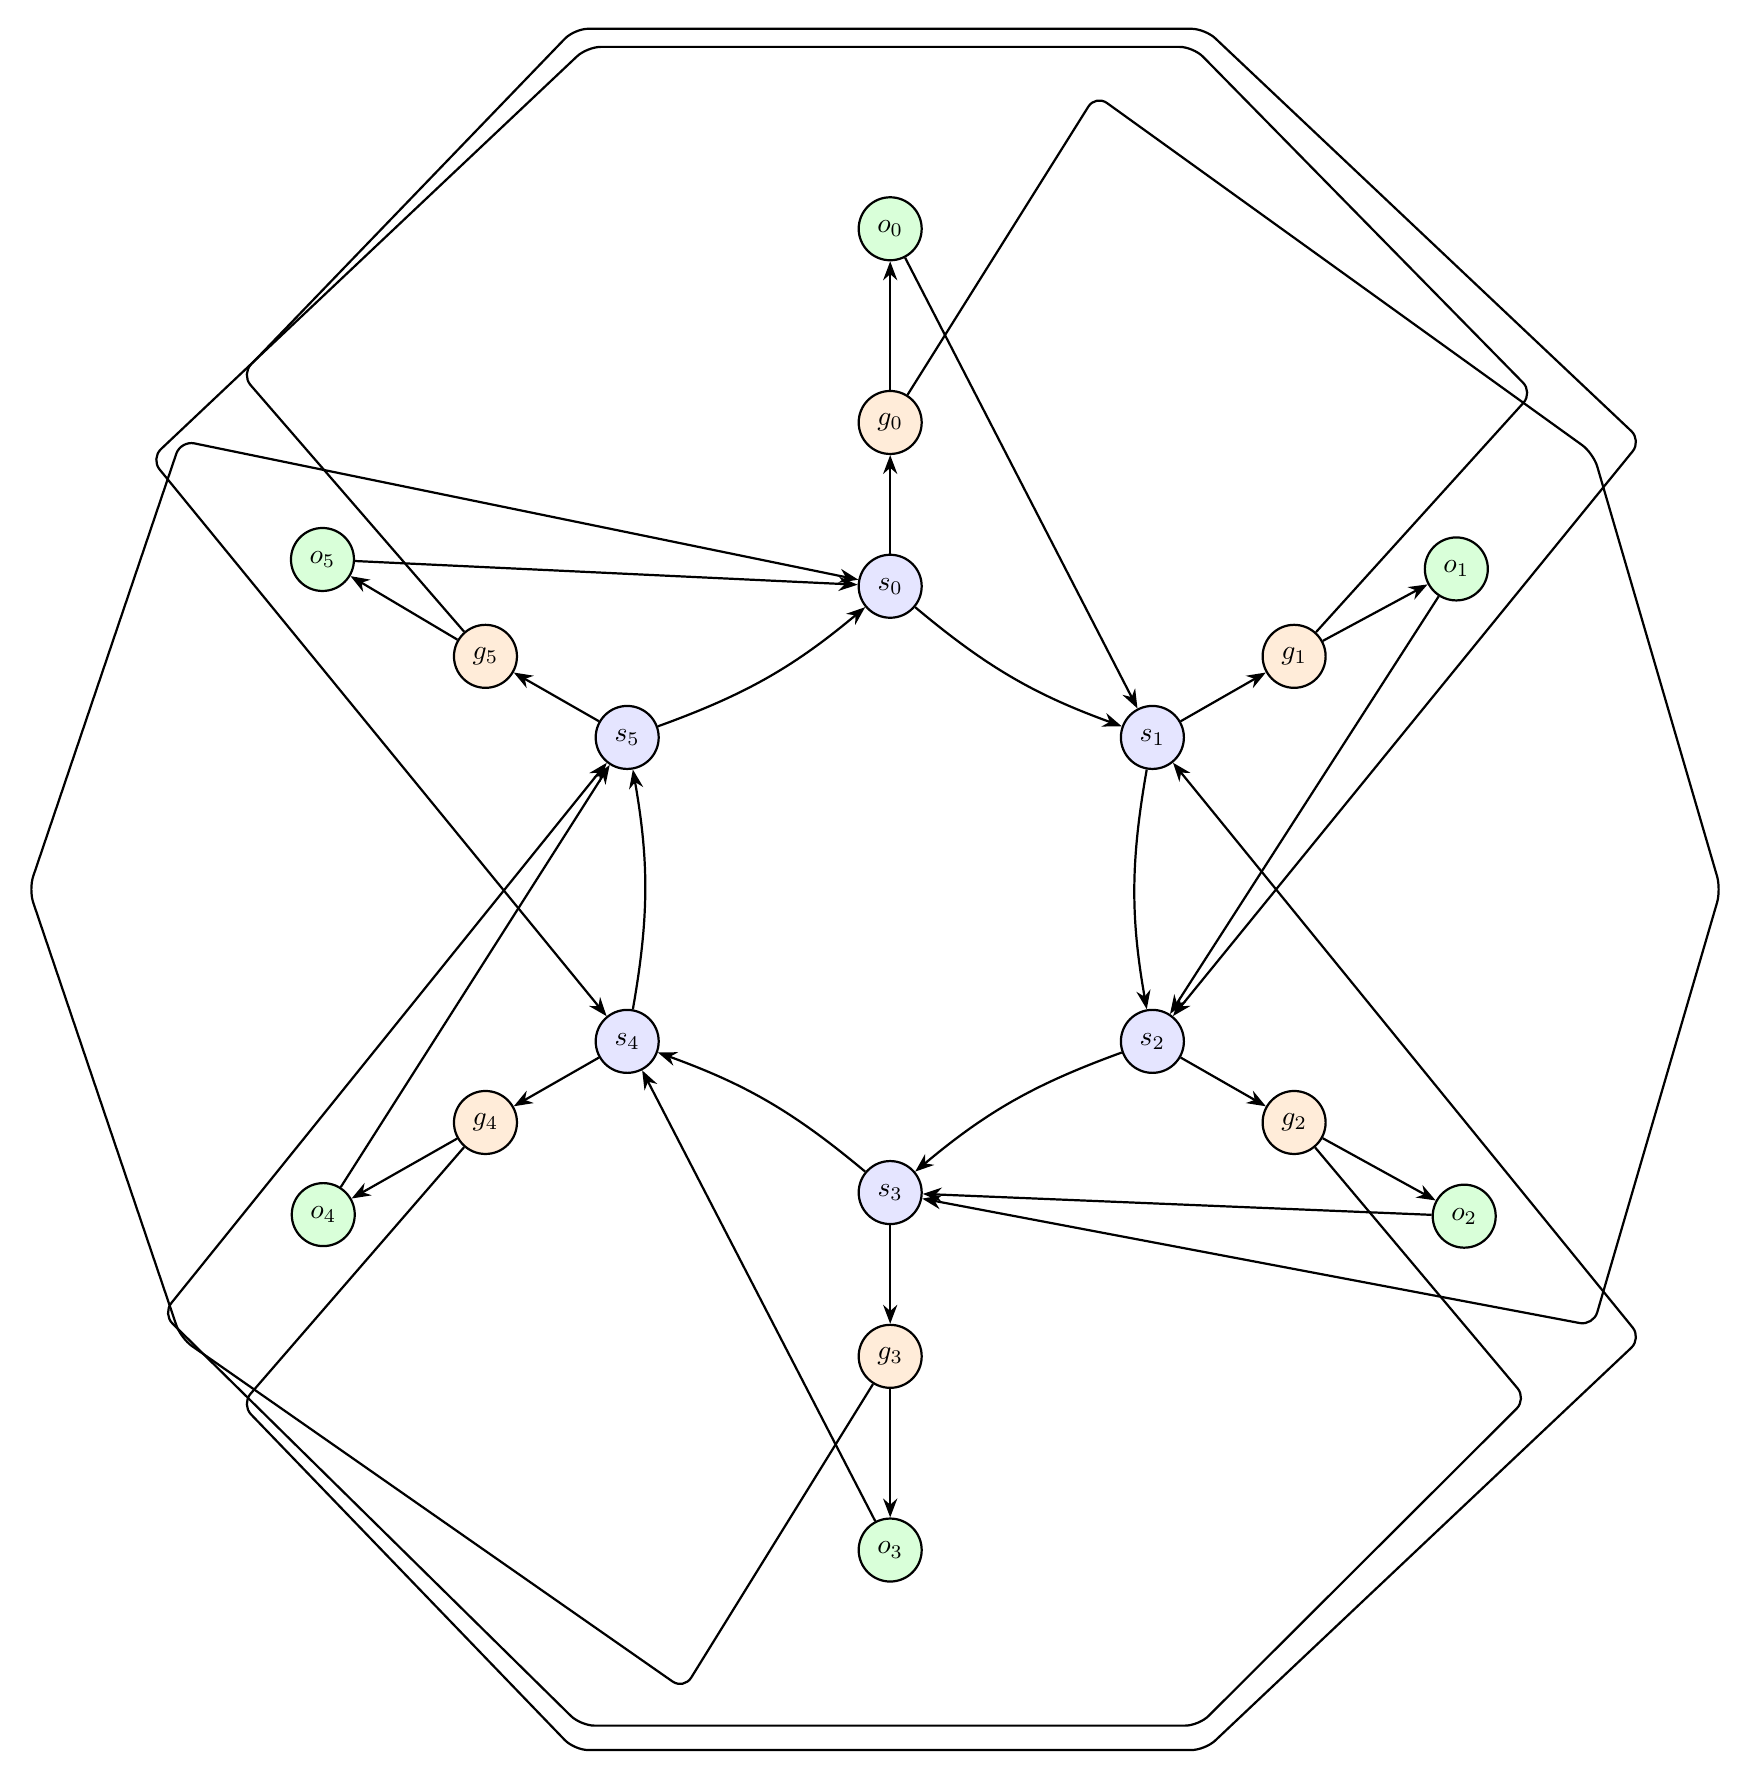
\begin{tikzpicture}[x=1cm,y=1cm]
\tikzset{
  graphnode/.style={circle,draw,thick,minimum size=8mm,inner sep=1pt,font=\sffamily},
  directed/.style={-{Stealth[length=2.4mm]},thick},
  undirected/.style={thick}
}
\node[graphnode,circle,draw,fill=blue!10] (n_s0) at (0.16,3.85) {$s_0$};
\node[graphnode,circle,draw,fill=blue!10] (n_s1) at (3.49,1.93) {$s_1$};
\node[graphnode,circle,draw,fill=blue!10] (n_s2) at (3.49,-1.93) {$s_2$};
\node[graphnode,circle,draw,fill=blue!10] (n_s3) at (0.16,-3.85) {$s_3$};
\node[graphnode,circle,draw,fill=blue!10] (n_s4) at (-3.18,-1.93) {$s_4$};
\node[graphnode,circle,draw,fill=blue!10] (n_s5) at (-3.18,1.93) {$s_5$};
\node[graphnode,circle,draw,fill=orange!15] (n_g0) at (0.16,5.93) {$g_0$};
\node[graphnode,circle,draw,fill=orange!15] (n_g1) at (5.29,2.96) {$g_1$};
\node[graphnode,circle,draw,fill=orange!15] (n_g2) at (5.29,-2.96) {$g_2$};
\node[graphnode,circle,draw,fill=orange!15] (n_g3) at (0.16,-5.93) {$g_3$};
\node[graphnode,circle,draw,fill=orange!15] (n_g4) at (-4.98,-2.96) {$g_4$};
\node[graphnode,circle,draw,fill=orange!15] (n_g5) at (-4.98,2.96) {$g_5$};
\node[graphnode,circle,draw,fill=green!15] (n_o0) at (0.16,8.39) {$o_0$};
\node[graphnode,circle,draw,fill=green!15] (n_o1) at (7.35,4.07) {$o_1$};
\node[graphnode,circle,draw,fill=green!15] (n_o2) at (7.45,-4.15) {$o_2$};
\node[graphnode,circle,draw,fill=green!15] (n_o3) at (0.16,-8.39) {$o_3$};
\node[graphnode,circle,draw,fill=green!15] (n_o4) at (-7.04,-4.13) {$o_4$};
\node[graphnode,circle,draw,fill=green!15] (n_o5) at (-7.05,4.19) {$o_5$};
\draw[directed] (n_s0) to[bend right=10] (n_s1);
\draw[directed] (n_s1) to[bend right=10] (n_s2);
\draw[directed] (n_s2) to[bend right=10] (n_s3);
\draw[directed] (n_s3) to[bend right=10] (n_s4);
\draw[directed] (n_s4) to[bend right=10] (n_s5);
\draw[directed] (n_s5) to[bend right=10] (n_s0);
\draw[directed] (n_s0) -- (n_g0);
\draw[directed] (n_g0) -- (n_o0);
\draw[directed] (n_o0) -- (n_s1);
\draw[directed] (n_s1) -- (n_g1);
\draw[directed] (n_g1) -- (n_o1);
\draw[directed] (n_o1) -- (n_s2);
\draw[directed] (n_s2) -- (n_g2);
\draw[directed] (n_g2) -- (n_o2);
\draw[directed] (n_o2) -- (n_s3);
\draw[directed] (n_s3) -- (n_g3);
\draw[directed] (n_g3) -- (n_o3);
\draw[directed] (n_o3) -- (n_s4);
\draw[directed] (n_s4) -- (n_g4);
\draw[directed] (n_g4) -- (n_o4);
\draw[directed] (n_o4) -- (n_s5);
\draw[directed] (n_s5) -- (n_g5);
\draw[directed] (n_g5) -- (n_o5);
\draw[directed] (n_o5) -- (n_s0);
\draw[directed,rounded corners=5pt] (n_g0) -- (2.77,10.09) -- (9.09,5.54) -- (10.71,0.00) -- (9.09,-5.54) -- (n_s3);
\draw[directed,rounded corners=5pt] (n_g1) -- (8.32,6.31) -- (4.01,10.70) -- (-3.69,10.70) -- (-9.23,5.47) -- (n_s4);
\draw[directed,rounded corners=5pt] (n_g2) -- (8.24,-6.47) -- (4.08,-10.62) -- (-3.77,-10.62) -- (-9.08,-5.39) -- (n_s5);
\draw[directed,rounded corners=5pt] (n_g3) -- (-2.46,-10.16) -- (-8.85,-5.70) -- (-10.78,0.00) -- (-8.85,5.70) -- (n_s0);
\draw[directed,rounded corners=5pt] (n_g4) -- (-8.08,-6.54) -- (-3.85,-10.93) -- (4.16,-10.93) -- (9.70,-5.70) -- (n_s1);
\draw[directed,rounded corners=5pt] (n_g5) -- (-8.08,6.54) -- (-3.85,10.93) -- (4.16,10.93) -- (9.70,5.70) -- (n_s2);
\end{tikzpicture}
\end{document}
